\section{Some Historical Background}
    \subsection*{The Ether}
        \indent
        Light with different polarizations cannot be made to interfere; hence light has to be a transverse wave. Light can move in the absence of a medium. Waves have to be propagating through a medium, so the medium that light propagates through was defined as the \textit{ether}, or the \textit{luminiferous aether}. 
        \newline \indent
        The Ether must be infinitely rigid so that it would not undergo compression and rarefaction (characteristics of longitudinal waves).
    \subsection*{How to Measure Earth's Speed through the Ether}
        \begin{center}
            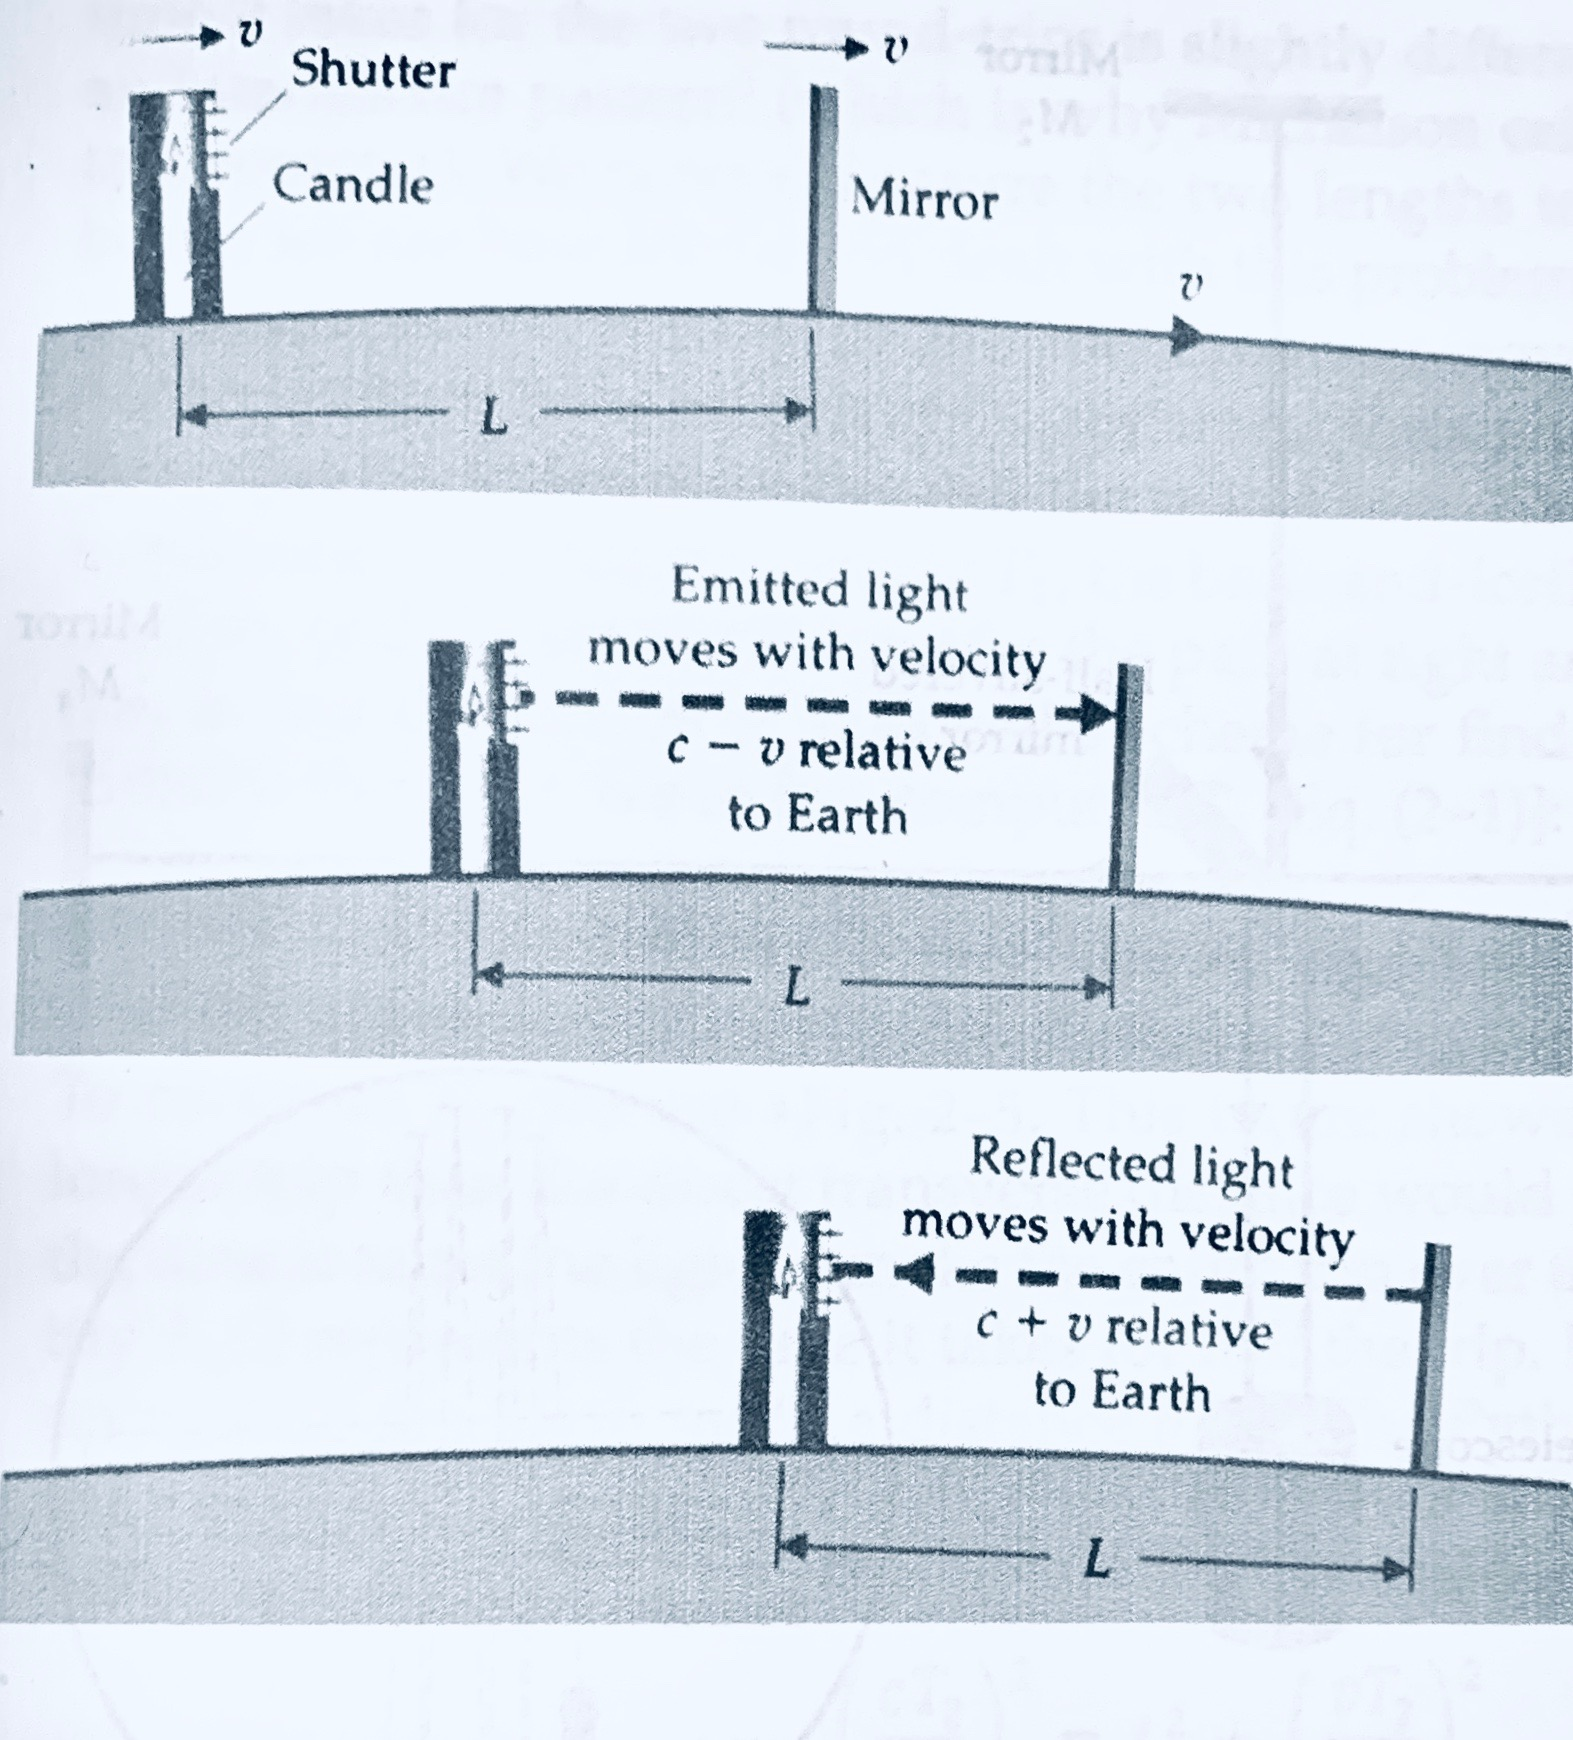
\includegraphics[width=180pt]{candleMirror.jpg}
        \end{center}
        Light is traveling from the candle to the mirror and back. If the Earth is not moving relative to the ether at speed $v$, the round trip time for the light (resting time) is $T = (2L) / c$. Now if the candle and mirror are stuck to the Earth, which is moving at $v$. The light will move at $c$ in the ether, $c - v$ going to the mirror, and $c + v$ coming back. Using this the total round trip time (moving time) is
        \begin{equation*}
            \frac{L}{c-v} + \frac{L}{c+v} = \frac{2L}{c}\frac{1}{1 - v^2/c^2} \approx \frac{2L}{c}(1 + v^2/c^2)
        \end{equation*}
        That approximation can be used since if $x$ is small then $1/(1 - x) \approx 1 + x$. Maxwell thought this would require too precise measurements to actually measure.
    \subsection*{The Michelson-Morley Experiment}
        Michelson wanted to prove Maxwell wrong.
        \begin{center}
            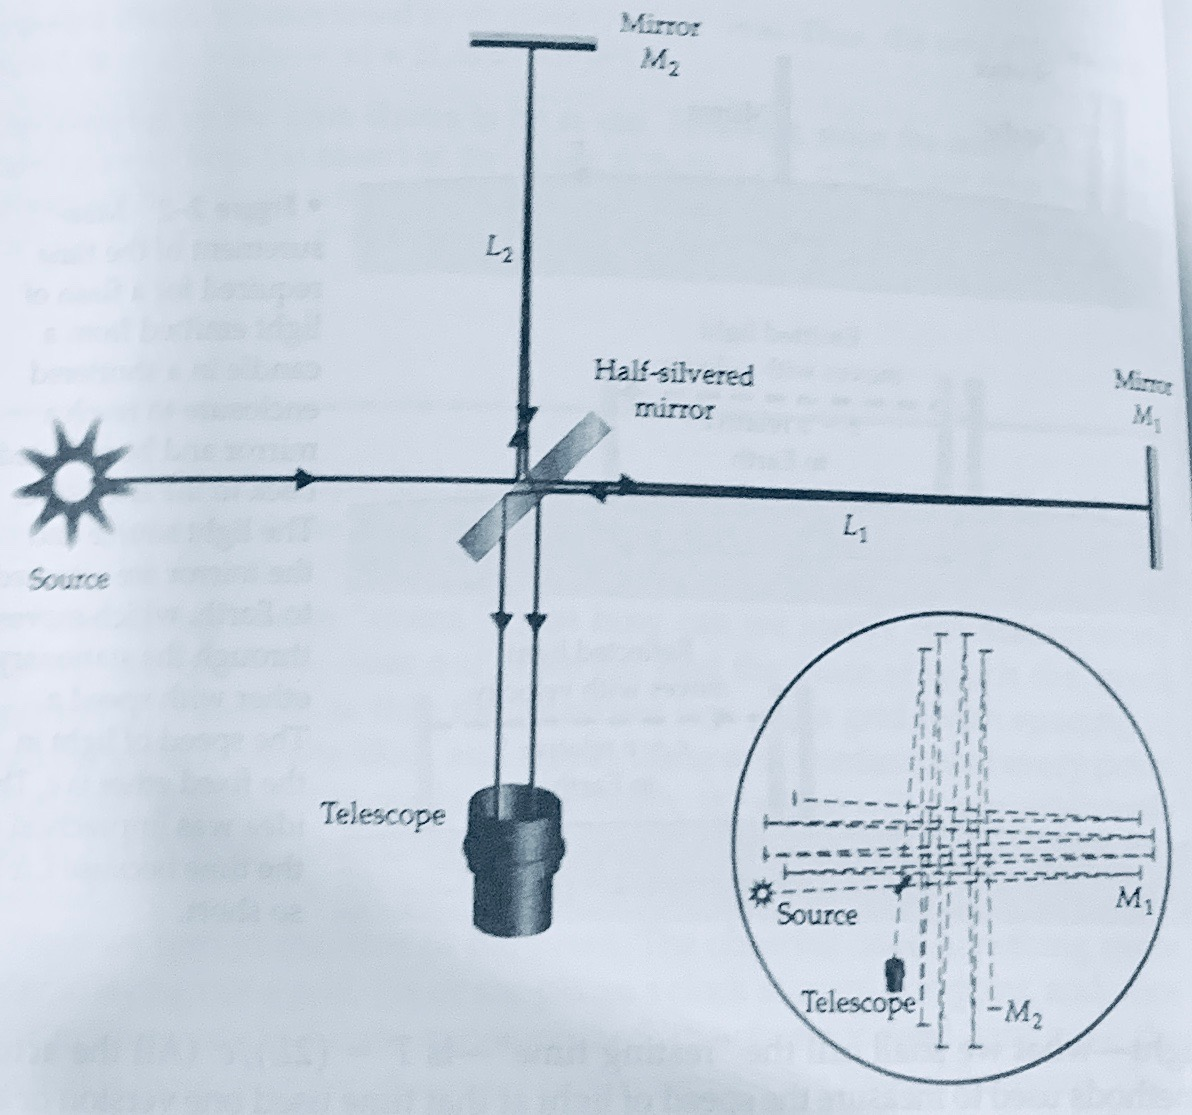
\includegraphics[width=230pt]{interferometer.jpg}
        \end{center}
        Since there is no way to precisely make the mirrors the same distance apart the split light waves will combine at the telescope at different times since the traveled different lengths. 
        \begin{equation*}
            \Delta T_{\text{rest}} = \frac{2L_1}{c} - \frac{2L_2}{c}
        \end{equation*}
        where the subscript "rest" refers to the fact that the apparatus is at rest in the ether. This time difference will cause a relative phase shift and interference.
        \newline \indent
        Now consider the system in motion at a constant speed $v$ in the $x$-direction. The travel time $T_1$ for the path along $L_1$ (parallel to the motion) is given by
        \begin{equation*}
            T_1 = \frac{2L_1}{c} \frac{1}{1-v^2/c^2} \approx \frac{2L_1}{c} (1 + \frac{v^2}{c^2})
        \end{equation*}
        with the same logic as from measuring the Earth's speed relative to the ether.
        \begin{center}
            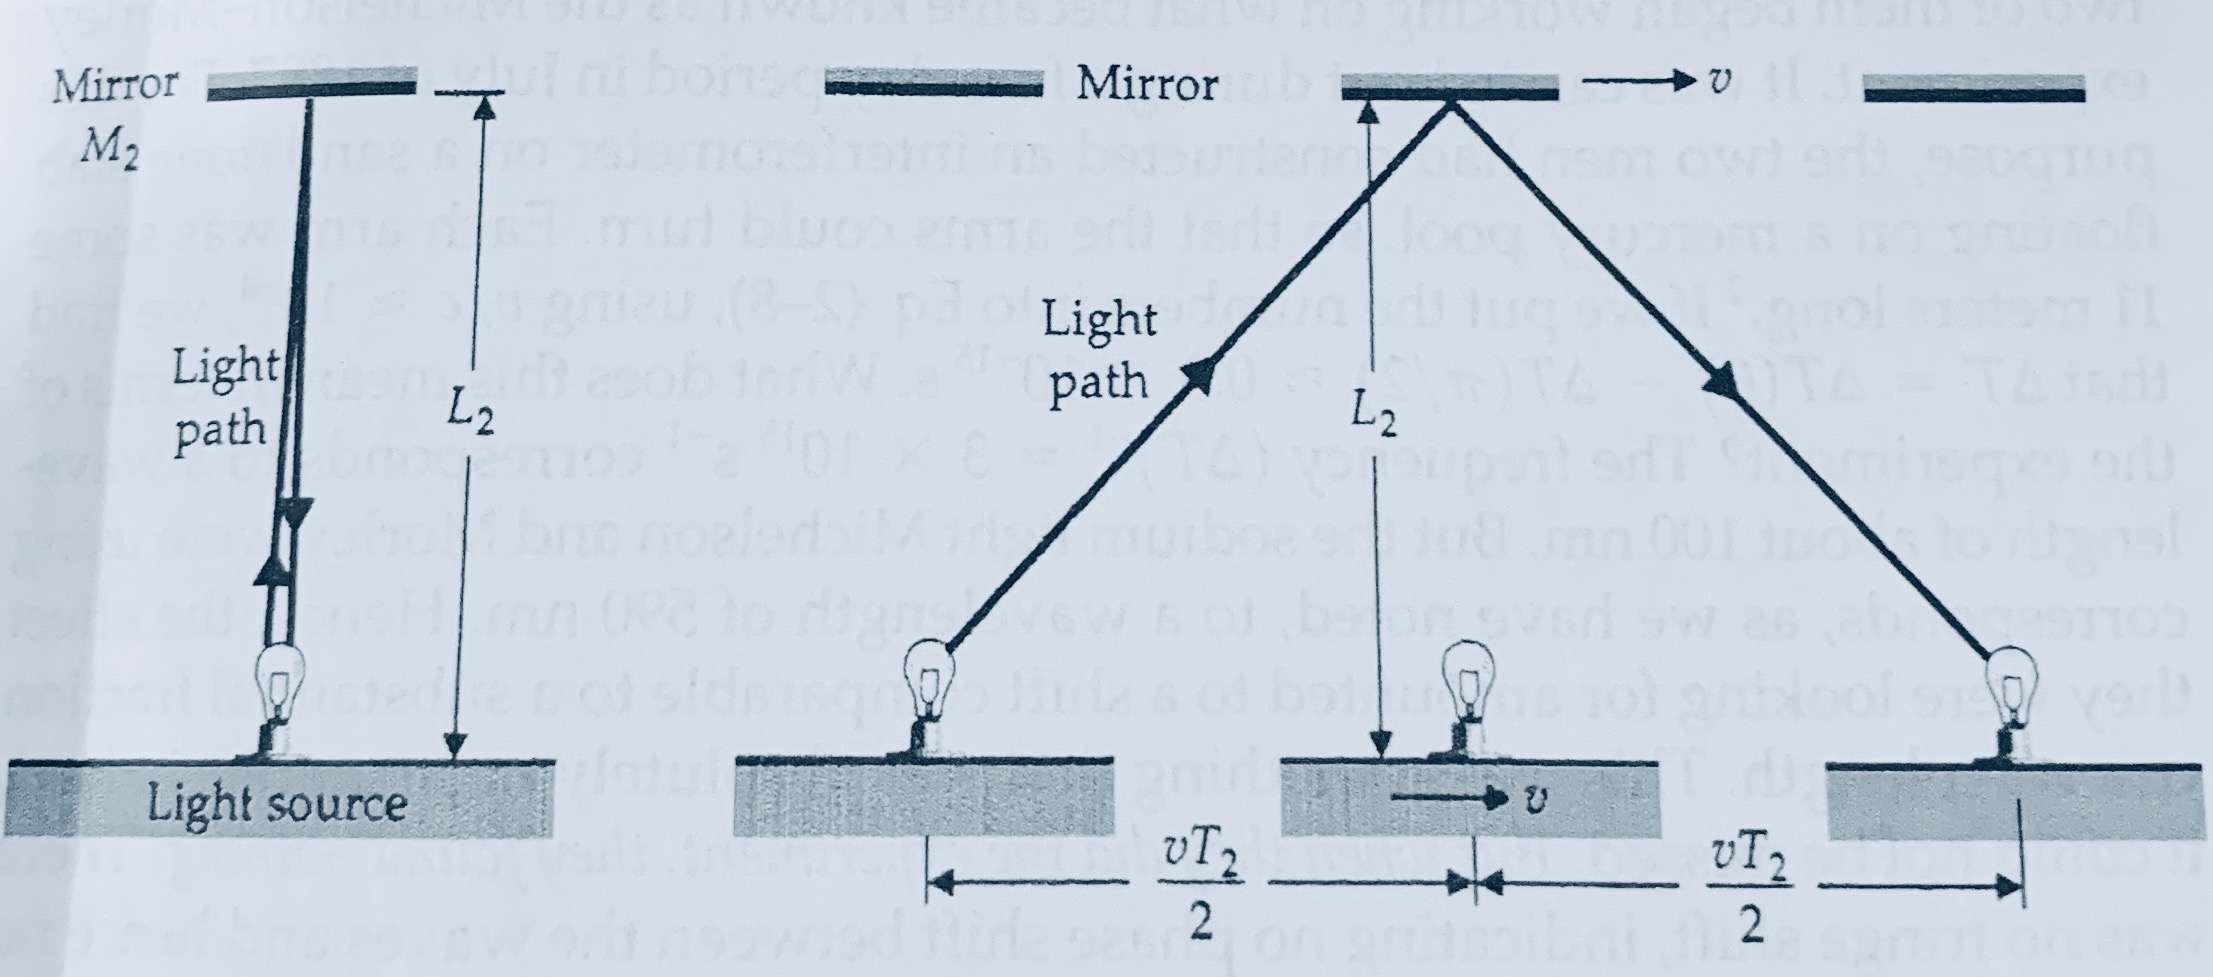
\includegraphics[width=240pt]{movinginterferometer.jpg}
        \end{center}
        $T_2$, the time for the path perpendicular to the motion, is given by the figure above.
        \begin{equation*}
            (\frac{cT_2}{2})^2 = L_2^2 + (\frac{vT_2}{2})^2
        \end{equation*}
        \begin{equation*}
            T_2 = 2L_2 / \sqrt{c^2 - v^2}
        \end{equation*}
        This results in an observer on Earth to see an effective speed of light as $$c' = \sqrt{c^2 - v^2}$$
        \begin{equation*}
            T_2 = \frac{2L_2}{c}\frac{1}{\sqrt{1 - v^2/c^2}} \approx \frac{2L_2}{c}(1 + \frac{v^2}{2c^2})
        \end{equation*}
        let $\Delta T(0) \equiv T_1 - T_2$.
        \begin{equation*}
            \Delta T(0) \approx \Delta T_{\text{rest}} + \frac{v^2}{c^2}\frac{2L_1-L_2}{c}
        \end{equation*}
        where $\Delta T_{\text{rest}} = 2(L_1 - L_2) / c$. $\Delta T_{\text{rest}}$ is dependent on precise measurements of $L_1$ and $L_2$ since it uses their difference.
        \newline \indent
        Now, if we rotate this setup so that $L_2$ is parallel to the motion and $L_1$ is perpendicular, you get
        \begin{equation*}
            \Delta T(\pi / 2) \approx \Delta T_{\text{rest}} + \frac{v^2}{c^2}\frac{L_1 - 2L_2}{c}
        \end{equation*}
        where $\Delta T(pi / 2)$ is the time in this configuration (it is rotated by $\pi /  2$). To cancel out $\Delta T_{\text{rest}}$ since it requires the precise measurements we will find the difference of the differences.
        \begin{equation*}
            \Delta T = \Delta T(0) - \Delta T(\pi / 2) = \frac{v^2}{c^2}\frac{L_1 + L_2}{c}
        \end{equation*}
        When performing the Michelson-Morley experiment they used light of a wavelength 590 nm, but they got a $\Delta T$ that corresponded with 100 nm.
        \newline \indent
        After triple checking, they came to the conclusion that the experiment did not work properly since light did not travel through a medium and the speed of light is the same, no matter the frame of reference.
    \subsection*{The Lorentz-Fitzgerald Length Contraction}
        Writing out $\Delta T$ without the approximations yields,
        \begin{equation*}
            \Delta T = \frac{2L_1}{c} \frac{1}{1 - v^2/c^2} - \frac{2L_2}{c} \frac{1}{\sqrt{1 - v^2/c^2}} - \frac{2L_1}{c} \frac{1}{\sqrt{1 - v^2/c^2}} + \frac{2L_2}{c} \frac{1}{1 - v^2/c^2}
        \end{equation*}
        For $\Delta T$ to be 0, the lengths in the first and fourth terms (terms in parallel to motion) must contract by a factor of $\sqrt{1 - v^2/c^2}$. So if an object begins moving uniformly in the direction of its length with a speed $v$, its length changes to $$L(v) = L(0)\sqrt{1 - v^2/c^2}$$ This is known as the \textbf{Lorentz-Fitzgerald length contraction}, or just \textbf{length contraction}. 
        